\begin{frame}{Dataset: overview}
\begin{center}
\begin{block}{\textbf{Stanford GitHub Social Networks dataset \cite{rozemberczki2019multiscale}}}
    \begin{itemize}
        \item A graph where nodes represent developers, and edges are mutual follower relationships between them
        \item Each node is assigned a label as ML or web developer derived from the job title of each user
        \item only developers who have starred at least 10 repositories are considered in dataset
        \item The graph is represented in a form of edge list
        \item Each node also contains its features vector
    \end{itemize}
To conduct the experiments, the dataset was split into train and test set in proportion of \textbf{8/2}
\end{block}
\end{center}
\end{frame}

\begin{frame}{Dataset: specification}
\begin{columns}
    \begin{column}{0.4\textwidth}
        \begin{itemize}
            \item \textbf{Balanced:} No 
            \item \textbf{Directed:} No 
            \item \textbf{Nodes:} 37700
            \item \textbf{Edges:} 289,003
            \item \textbf{density:} 0.001
        \end{itemize}
        
    \end{column}
    \begin{column}{0.6\textwidth}
        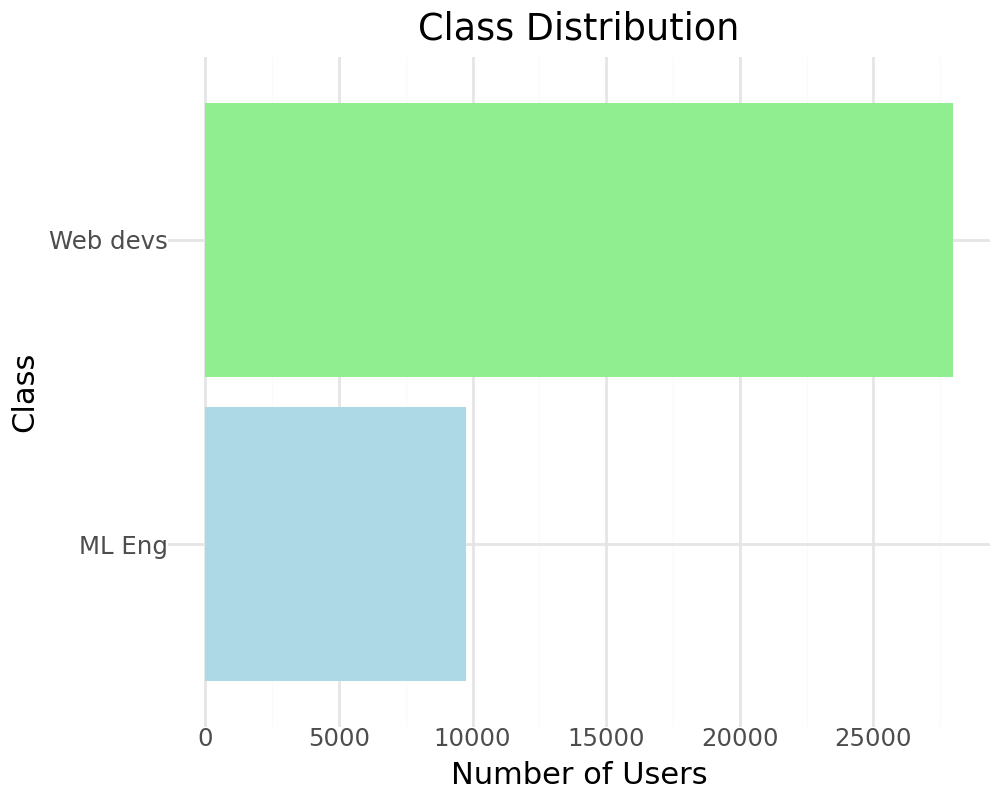
\includegraphics[width=1\textwidth]{images/imbalanced.png}
    \end{column}
\end{columns}
\end{frame}